% v2-acmsmall-sample.tex, dated March 6 2012
% This is a sample file for ACM small trim journals
%
% Compilation using 'acmsmall.cls' - version 1.3 (March 2012), Aptara Inc.
% (c) 2010 Association for Computing Machinery (ACM)
%
% Questions/Suggestions/Feedback should be addressed to => "acmtexsupport@aptaracorp.com".
% Users can also go through the FAQs available on the journal's submission webpage.
%
% Steps to compile: latex, bibtex, latex latex
%
% For tracking purposes => this is v1.3 - March 2012

\documentclass[prodmode,acmtosem]{acmsmall} % Aptara syntax

% Package to generate and customize Algorithm as per ACM style
\usepackage[ruled]{algorithm2e}
\usepackage{textcomp}
\usepackage{gensymb}
\usepackage[utf8]{inputenc}
\usepackage[table]{xcolor}
\usepackage{natbib}
\usepackage{subfigure}
\usepackage{tabularx}

\renewcommand{\algorithmcfname}{ALGORITHM}
\SetAlFnt{\small}
\SetAlCapFnt{\small}
\SetAlCapNameFnt{\small}
\SetAlCapHSkip{0pt}
\IncMargin{-\parindent}

% Metadata Information
% \acmVolume{9}
% \acmNumber{4}
% \acmArticle{39}
% \acmYear{2010}
% \acmMonth{3}

% Copyright
%\setcopyright{acmcopyright}
%\setcopyright{acmlicensed}
%\setcopyright{rightsretained}
%\setcopyright{usgov}
%\setcopyright{usgovmixed}
%\setcopyright{cagov}
%\setcopyright{cagovmixed}

% DOI
%\doi{0000001.0000001}

%ISSN
%\issn{1234-56789}

% Document starts
\begin{document}

% Page heads
\markboth{}{Dynamic obstacle mapping for the visually impaired using sensor fusion.}

% Title portion
\title{Dynamic obstacle mapping for the visually impaired using sensor fusion.}
\author{Johann Thor Kristthorsson
\affil{University College London}
Ifeanyi Ndu
\affil{University College London}
Veselin Pavlov
\affil{University College London}
Shuang Zhang
\affil{University College London}
}
% NOTE! Affiliations placed here should be for the institution where the
%       BULK of the research was done. If the author has gone to a new
%       institution, before publication, the (above) affiliation should NOT be changed.
%       The authors 'current' address may be given in the "Author's addresses:" block (below).
%       So for example, Mr. Abdelzaher, the bulk of the research was done at UIUC, and he is
%       currently affiliated with NASA.

\begin{abstract}
Abstract goes here
\end{abstract}


%
% The code below should be generated by the tool at
% http://dl.acm.org/ccs.cfm
% Please copy and paste the code instead of the example below. 
%
% \begin{CCSXML}
% <ccs2012>
%  <concept>
%   <concept_id>10010520.10010553.10010562</concept_id>
%   <concept_desc>Computer systems organization~Embedded systems</concept_desc>
%   <concept_significance>500</concept_significance>
%  </concept>
%  <concept>
%   <concept_id>10010520.10010575.10010755</concept_id>
%   <concept_desc>Computer systems organization~Redundancy</concept_desc>
%   <concept_significance>300</concept_significance>
%  </concept>
%  <concept>
%   <concept_id>10010520.10010553.10010554</concept_id>
%   <concept_desc>Computer systems organization~Robotics</concept_desc>
%   <concept_significance>100</concept_significance>
%  </concept>
%  <concept>
%   <concept_id>10003033.10003083.10003095</concept_id>
%   <concept_desc>Networks~Network reliability</concept_desc>
%   <concept_significance>100</concept_significance>
%  </concept>
% </ccs2012>  
% \end{CCSXML}

% \ccsdesc[500]{Computer systems organization~Embedded systems}
% \ccsdesc[300]{Computer systems organization~Redundancy}
% \ccsdesc{Computer systems organization~Robotics}
% \ccsdesc[100]{Networks~Network reliability}


\keywords{Sensor Fusion, Software Engineering,
Visually Impaired, Blind, Microsoft}

\acmformat{Johann Thor Kristthorsson, Ifeanyi Ndu, Veselin Pavlov and Shuang Zhang, 2016.}


\begin{bottomstuff}
This work was made in collaboration with Microsoft and the Guide Dogs association.
\end{bottomstuff}

\maketitle

\section{Introduction}
Two million people are living with visual impairment in the UK and despite that indoor environments are often not designed for this vast group of individuals in mind. ~\cite{NHSBlindStatistics} This means that the visually impaired have to depend on mobility tools to make their way around their environment. Mobility canes and guide dogs are the most important ones but are limited in their use. The canes have restricted use to a person needing to navigate from place to place, and the guide dogs are not currently available to assist all visually impaired persons in the UK. The Guide Dogs Association is working towards the goal of providing as many people with guide dogs as possible but is not able to meet the demand. The project falls under the Cities Unlocked umbrella, an initiative that was started to respond to the lack of available guide dogs in the UK ~\cite{CitiesUnlockedGeneral}. Cities Unlocked has recently been moving more towards improving and enriching the experiences of the visually impaired, rather than focusing solely on their mobility.

Microsoft has been exploring different technologies that could help the visually impaired in their day to day lives and wanted to elicit the help of UCL in this exploration. A team of 8 MSc students, 4 from software systems engineering and 4 from computer science was put together, and one member was appointed as the team leader. To clarify the specific topic of the project, several brainstorming sessions were held to explore the aims and goals. The specific field of study that the clients wanted the team to explore was the use of wearable sensors that could be utilised by the visually impaired. Additionally, the clients wanted to use cheap, off the shelf, hardware and use a technique called sensor fusion to maintain accuracy~\cite{SensorFusion}. Generally speaking sensor fusion is any processing method that combines sensor readings from disparate sources into a result that has less uncertainty than the constituent sources. 
After exploring several possible use cases for these technologies the client and the UCL team decided to find a way to improve the experience of the members of the visually impaired population when entering specific indoor environments.
Specifically in environments that are unfamiliar to the user and that are not equipped with any particular navigation infrastructure. There has already been thorough research done on indoor navigation, but the identification of obstacles seemed to be a good fit for the hardware and technology requirements of the client.
%TODO: Don't cite wikipedia

\section{Literature review} % TODO: Change to background
% TODO: Check if there is a difference in font size.
% TODO: use the 
% TODO: citet and citep
Obstacle detection is a large topic and has been popular in the last few years with the advent of autonomous vehicles and unmanned aerial vehicles.
The Defence Advanced Research Project Agency (DARPA) in the United States has held several competitions to push the research community towards this particular topic. The DARPA Grand Challenge in 2005 and the Urban Challenge in 2007 offered millions of dollars in prizes and sparked considerable interest within the research community~\cite{DARPAGrandChallenge2005,DARPAUrbanChallenge2007}.
\subsection{Obstacle detection}
In the specific case of obstacle detection as an assistive technology, there have been several papers exploring the topic. \citet{Cardin2007} developed a wearable system that uses an array of ultrasonic transducers to do sonar sensing of obstacles around a subject. The subject is notified of the obstacles through vibrotactile instruments sewn into clothing around the subject's torso. Experiments were conducted by blindfolding test subjects and having them navigate an environment filled with obstacles. The time it took the subjects to navigate was recorded, and the use of the system resulted in a 50\% reduction in navigation time after a short training time~\cite{Cardin2007}. The system developed by \citet{Shin2007} is similar to \citet{Cardin2007} but adds audible feedback through a headset~\cite{Shin2007}. These methods are entirely reactive, in that they sense and identify obstacles in space but do not record its position for possible future use. In addition to this, the evaluation of the detection accuracy is lacking. The studies do not describe their experimental setups accurately, and the data collection methods are never mentioned.
%These types of methods are common and widely explored both for the purposes of small robots and autonomous vehicles ~\cite{Kato2002}. 
%Shoval et al. have made attempts to fuse the work done in autonomous driving and robotics with the work in assistive technologies. They did this by mounting sonar sensing hardware on a robot that serves the same purpose as a guide dog. It has one axle and wheels that are powered. The robot is pushed by the subject via a handle, the robot can then detect and avoid obstacles and the subject notices the change in the robots movements through the handle ~\cite{Shoval2003}.
\subsection{Sensor Fusion}
Sensor fusion, or cooperative fusion, is a well-known term in the context of obstacle detection and navigation. This kind of technique combines the data from several sensors to get a more certain result than using sensors individually. \citet{Labayrade2005} describe algorithms and architectures that facilitate cooperative fusion of two different kinds of sensors, stereovision and LIDAR to detect obstacles in an autonomous driving scenario~\cite{Labayrade2005}. Cooperative fusion is used to detect barriers in the road in front of a vehicle and determine its distance with good accuracy. The use of sensor fusion decreased the rate of false negatives in the detection from 14.7\% and 5.2\% for LIDAR and stereovision respectively, down to 5.2\%. In addition the rate of false negatives went down from 4.5\% and 3.2\% respectively to 1.2\%. \citet{Cho2014} reached similar results showing an increase in the rate of true positives in obstacle detection from 83.2\% to 89.9\% by using fusion instead of using actual sensor values~\cite{Cho2014}. Contrary to the research found for the use cases for the visually impaired these papers provide a thorough explanation of the evaluation and data gathering performed and will prove useful in designing the evaluation strategy for this project. These methods have been developed specifically for use in the scenario of autonomous driving but are directly applicable to the scenario of detecting obstacles around a visually impaired pedestrian. Sensor fusion was introduced into the Windows 8 Operating system to provide stability to applications relying on clean and stabilised data. \citet{Gear2012} described a situation where engineers at Microsoft attempted to map a 3D virtual environment to a real environment in an app running on a tablet. First of all they tried emulate up and down movements in the virtual environment using an accelerometer. Almost immediately they encountered an issue when tilting the tablet and holding the tablet in a stationary position. Noise coming from the accelerometer alone caused jittery movements in the applications. To achieve a much more stable movement, the accelerometer readings was passed through a low-pass filter. The low-pass filter fulfilled its duty but simultaneously introduced a bottleneck into the app. Movement was significantly smoother but the motion in the app felt unresponsive and sluggish. The engineers also used a 6-axis compass which is a 3D accelerometer and 3D magnetometer to emulate left and right movements however it did not yield practicable result due to the instability of the 6-axis sensor. Finally the engineers hit a breakthrough with sensor fusion using the 3D accelerometer, 3D magnetometer and 3D gyroscope. Data collected from all 9-axis resulted in a smooth and fluid experience in the virtual app. Additionally the sensors complemented each other in terms of areas where they fell short~\cite{Gear2012}.

In light of research described in the literature reviewed the team will be able to reach the aims mentioned above of this project by developing a data collection platform that gathers data from many different cheap sensors. The sensor data will be used to identify obstacles, and the accuracy of the results will be increased by using sensor fusion.



% Add aims and goals
% What are we building now and what are it's aims
\section{Proposed System}
% TODO: make a good argument for how we managed RISK
\subsection{Preliminary work}
\label{sec:Prelim}
% How did we end up with our current aim
% US sensors and why we discarded those.

% Subsection this into VI obstacle detection and Sensor fusion, then bring back together.

%TODO: citation 

The initial plan for this project was to make use of device developed by students in the Electrical Engineering department. The hardware consists of an armband that can detect ultrasonic frequencies. Those frequencies are emitted by at least 3 beacons in strategically predefined locations in the room. The armband, in conjunction with a computer and an Android device, then triangulates the position of the armband in space.
The former use cases to be explored focused on detecting gestures and possible indoor location possibilities. However, soon after the project was presented to the team, the hardware was found to have several limitations. The team found that the location accuracy was considerably less than what was initially described. The initial description of the hardware stated that the location accuracy was sub-centimetre, which is the theoretical minimum, but the functional accuracy was between 10 and 50 centimetres. This eliminates the gesture use case since more precision is needed to get accurate gesture recognition.
%TODO: citation
Furthermore, the hardware can only function if 3 beacons are within a 130\degree cone in front of the receiver. This severely limits the practicality of the device for indoor location since a wearable piece of hardware is usually blocked by the wearer's body in addition to any obstacle in the environment such as static or movable objects.
%TODO: citation
Therefore the high probability of getting unacceptable performance out of the hardware platform was found to cause too much risk to the project and the team mitigated that risk by pivoting the focus of the project to a different topic.

\subsection{Stakeholders and Project Context}
To identify and prioritise the goals and objectives of the SSE team first enumerated the stakeholders of the project and their desired outcomes. This would prove valuable to maintain a clear vision throughout the development process and to limit the risk of non-acceptance later on in the project.

\subsubsection{Microsoft}
Microsoft is both the sponsor and the client in this project, in addition to that Microsoft provides the team with access to domain experts and other resources. The primary outcome that Microsoft wants from the project is research into available assistive technologies based on obstacle detection and sensor fusion. The team is therefore responsible for conducting that research, enumerating the technologies available and developing a proof of concept prototype to illustrate the possibilities of a system using them.
Mr Jarnail Chudge is representing Microsoft and will be the team's client for the duration of the project.

\subsubsection{Academic}
The academic administrators and supervisors of this project have a specific vision for how the team should apply their knowledge to the development process and client communication.
The outcomes the academic stakeholders are interested in are having the team maintain rigorous documentation of the project, upholding the state of the art software engineering processes and maintaining good communication with the client throughout the process.

\subsubsection{Team members}
The team members have a different stake in the project since they want, not only, a good mark but also a rewarding learning experience.
They want to see the project fulfilling the requirements of the other stakeholders while also getting a chance to tackle interesting and challenging problems that will widen their knowledge base in the field of Software Engineering.
To ensure a passing mark for every member of the team, the SSE team aims to minimise the overall risk of the project and put in place contingencies in the event of possible non-acceptance of the project.

\subsection{High level goals}
The team's initial contact with the client was a brainstorming session where he expressed the vision for the project. He expressed Microsoft's desire to have an end product which would feel natural to the user with very little work on the user's part regarding getting themselves familiar with the product. Then they raised the idea of using a sensor or combination of wearable sensors to achieve the ultimate goal. Ideas were then bounced around, and a subject area was found that was open for research and of value to our client.
Microsoft Research has done some investigation into using sensor fusion and wanted to see how that technology could be utilised in aiding the visually impaired~\cite{Gear2012}.

After the brainstorming session, the team met several times to brainstorm further and research possible applications around the sensor fusion concept and decided on a few possible project proposals.
These were presented to the client, and he expressed interest in continuing with one of them.
For the final project proposal, our client agreed on a research area that will help the visually impaired navigate an indoor environment.
By using sensor fusion the team was to build a system that could collect data from various disparate sensors and identify the location of the user and obstacles in its environment.

The goal is to use cheap, off-the-shelf sensors and mitigate any error in the sensor readings by correlating different readings. This will help us reduce error and increase accuracy by using sensor fusion methods. The ones the team has selected to examine are the use of a Kalman filter, the central limit theorem and neural networks, in that order, to evaluate their applicability to the problem space. In order to identify the main goals of our client the team came up with scenarios and use cases, within the scope that was mentioned in section~\ref{sec:Prelim}, and presented them to the client. This was followed up by a discussion that leads to the identification of the following high level goals.


The main objective was to improve the experience of the visually impaired in a specific scenario. The scenario in question involved a visually impaired individual entering a space like a coffee shop and having to navigate around obstacles like tables and chairs.
This made obstacle detection a clear objective and secondary objectives relating to that were then further explored. The use of the obstacle detection in conjunction with detection of points of interest was discussed as a possible objective but was deemed less important by the client.
The use of Open Street Maps was discussed in this context as a database to work from with regards to gathering information on points of interest~\cite{OSM}.
Another secondary objective that came up on the topic of obstacle detection was the use of sensor fusion. Members of the Microsoft Research team had shown interest in the team evaluating sensor fusion techniques in the context of obstacle detection. This objective was deemed essential since it fit well with the rest of the project.

% Goal model diagram
% \begin{figure}
% \label{fig:GoalModel}
% \centering
% 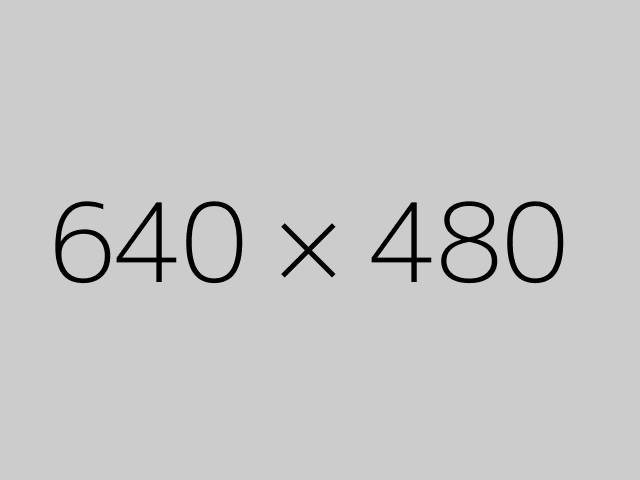
\includegraphics[width=\textwidth]{test640}
% \caption{An awesome goal model}
% \end{figure}

% TODO: Link to appendix with formal goal definitions

\subsection{Requirements}

Table \ref{table:1} shows a list of requirements our system will fulfil (please see section \ref{Appendix} for a full description of our requirement patterns).\\

\renewcommand{\arraystretch}{1.5}

\begin{center}
\begin{tabularx}{\textwidth}{| X | X |} 
 \hline
 \rowcolor{lightgray}
 \multicolumn{2}{|c|}{List of Requirements} \\ [0.5ex] 
 \hline\hline
 Identifying points of interest in the environment. &  Detecting obstacles \\
 \hline
 Feeding back mapping information &  Manually identifying obstacles in a space \\
 \hline
 Manually removing an obstacle from the map &  Providing navigation for a user to a point of interest \\ 
 \hline
 Voice interactions - listing &  Voice interactions - acceptance \\ 
 \hline
 Screen interactions - listing &  Screen interactions - acceptance \\ 
 \hline
 Classification of obstacles/Points Of Interest &  3D Directional Sound \\ 
 \hline
 Head Gestures &  IR and Ultrasound \\  
 \hline

 \hline
\end{tabularx}
\label{table:requirements}
\end{center}

\section{System Architecture}
\label{architecture}
Given the goals the team and the client set for this project, there were several considerations to be made to make the architecture flexible and performant enough to satisfy the requirements. Having the requirement of being able to accept data from many kinds of sensors made it clear that the architecture had to be made up of a variety of strategies to homogenise the data so that it could be processed in a more abstract way. Subsequent processing could then be performed based on a fixed data model that would make it easier to develop rapidly and evaluate different processing strategies.


\begin{figure}
\label{fig:architecture}
\centering
\includegraphics[width=\textwidth]{Architecture}
\caption{Temporary architecture figure}
\end{figure}


\subsection{Data collection}
\label{dataCollection}
The data collection aspect of the project was a major architectural concern since the data processing part of the pipeline is supposed to handle data coming from many different kinds of sensors. This part would have to be able to filter and make sense of a high volume of sensor readings and prepare them for further processing. Therefore the SSE team set up a simple, well documented, API for the data collection applications to communicate with. This decoupled the processing platform from the data collection by exposing an interface that clearly stated the data expected by the processing platform from the data collection applications.
The initial implementation plan for this part of the architecture was to have the CS students implement each of the data collection applications, and the SSE team would implement the processing platform.
Concern about this structure was raised by our academic stakeholders where they wanted the SSE team to decouple their work further from the CS students. This was done by having one of the data collection application implemented by the SSE team, thereby making the SSE team responsible for a full slice through the system. Any additional data collection by the CS students would therefore be additive and not essential to the success of the project.

\subsubsection{Visual obstacle detection}
One CS student was assigned the task of exploring the use of camera feeds to detect obstacles. The main aim of the task is to determine what specific method within the wide field of computer vision might fit best for obstacle detection. The two items that stood out were stereovision, which uses two cameras separated by a set distance, to detect the distance to each point in an image and use that to determine if there is an obstacle in the path. The second is to use colour detection to determine the floor area of a room and then mask out any parts of the image that are of a different colour, the masked out sections would then be identified as obstacles. The cameras were to be mounted on a headset and directed at an angle towards the ground in the direction the user was facing to detect obstacles in that area. The colour detection method provided the best results and was used to gather data for the mapping platform.

\subsection{Ultrasound and Infrared}
Another CS student worked on an application that polled cheap off-the-shelf infrared and ultrasound range finding sensors. These sensors would, like the computer vision cameras, make measurements of the objects in front of the user and send the readings to the obstacle mapping platform.

\subsection{Aggregation}  % TODO: find a good name for this
The API mentioned in Section~\ref{dataCollection} was the only contact point for the data collection applications. The component needed to be designed and implemented to handle large quantities of incoming readings, from many different sources, and efficiently buffer and pass them to the processing component. The aggregation component would group together readings and post them to the processing component in a producer/consumer pattern. To manage this the SSE team evaluated several message broker systems for the job, Apache Kafka, Azure EventHub and RabbitMQ. The criteria used was threefold, one was the applicability of the technology to the producer/consumer pattern, their cost and their ease of integration with the technology used in the processing component. Azure EventHub was considered as a robust and scalable possibility but was discarded because of the cost associated with running it for the duration of the project, see Appendix~\ref{ArchitectureCost}. RabbitMQ and Apache Kafka both fit well with the architecture and patterns the team had in mind but ultimately Apache Kafka was chosen because of it's ease of integration with Apache Spark.

Kafka is a distributed publish subscribe messaging service designed specifically to be fast and handle large volume of data inflow coming from various sources. Kafka is fault tolerant as it is inherently distributed over a cluster computers so if one broker fails, the other live brokers will complemenent the node. Kafka achieves fault tolerance with the help of zookeeper which is a seperate Apache tool for configuration and synchronisation of nodes in a distributed system. A leader in a kafka broker is resposnible for read/write operations in a partition and only one leader can exist for every partition. If a leader dies in the cluster, zookeeper is responisble for managing change in leadership to an existing slave broker. Furthermore Kafka seamlessly integrates with Spark for high speed data processing. 

\subsection{Processing}
With Apacha Kafka working as a producer for the producer/consumer pattern and Apache Spark working as the consumer the team managed to handle the level of throughput needed for the purposes of the project.
Spark consumes streams of sensor readings coming from Kafka in the distributed way, performs the processing on the data and stores the result into database.

\subsection{Storage and API}
The obstacles identified by the Spark stream processing are finally persisted in a database for further processing and use by the feedback applications. The database used for persistence needed to fulfil several requirements to fit the project, scalability with increased load, flexibility of schema and cost.
The scalability can be solved by most distributed databases but the flexibility of schema and cost are more difficult to work around.
The first step in the choice of database technology was to decide on a SQL or NoSQL database, where NoSQL provided the flexibility needed. After NoSQL was selected the next question was whether to go for a document storage or column storage database. Both provide a flexible schema data persistence but the data modelling needed for each is quite a bit different. After these deliberations there were 3 possibilities explored, Apache Cassandra, Azure DocumentDB and MongoDB.  Here again the cost of running an Azure product is prohibitive to an academic prototype project, in addition to that the documentation and troubleshooting resources of the open source technologies is far better than the ones available for Azure. Apache Cassandra and MongoDB both seemed to fit well with the needs of the architecture, both are easily integrated with Spark and both have more than adequate documentation. The deciding factor in choosing between the two was the fact that Cassandra is an Apache distributed system that inherently works with Zookeeper in the same way that Spark and Kafka do. This meant that the time and effort in setup and maintenance would be lessened since all these technologies run in the same managed distributed environment.

\subsection{Feedback}
After Processing, the obstacle data will be stored in Cassandra database. Based on the Requirement mentioned in Section 3.4, we implement the feedback part to show the user the surroundings by querying the stored obstacle data. When to query the nearby obstacles in the database, we set the query based on the user‘s location data which consists of latitude, longitude and radius. In an actual situation where our platform is used for, we show the obstacles nearby instead of all the obstacles detected and stored. For this reason, we set radius which allows the platform give user feedback within an exact area. We show the obstacle both in a scrollable list and on a visual map.

% TODO: make a good argument for how we managed RISK

\section{Implementation}
As described in section~\ref{architecture} the chosen architecture uses a variety of different technologies to achieve its goal. Each component therefore had a predefined best practice in implementation. The team aimed to follow best practices when working with each technology and align their work so that each member would be able to work on each component interchangeably.

The first concern the SSE team took on was the choice of programming language. Each of the Apache technologies supported Java, Scala and Python for development so those were the options evaluated. Java and Scala are the most common implementation languages for these technologies and provide the most comprehensive documentation and support. The team felt more comfortable with Java than Scala and the choice of using Android for the front end applications drove the decision towards using Java for the server side as well. This would help the team work together in an environment everyone was comfortable with and limit the risk posed to the project that comes with the team learning a new environment during development.

\subsection{Android app and Jar file}
A socket on our VPS will be listening indefinitely on a particular port for incoming data from our various sensing hardware. Each sensor or combination of sensors will measure data, do some preprocessing before sending data across to our VPS over a UDP connection. For instance one of the CS students would send three distance estimates based on the measurements collected from 2 ultrasound and 1 infrared sensor.

\subsection{Kafka Producer Listener}
At the listening end we would essentially do a partial deserialisation of the data packet into a JSON object to obtain the topics from each packet. Afterwards the JSON object is published into the kafka cluster.

%Describe
\subsection{Spark}
After Kafka has indexed, filtered and sorted the sensor readings into topics, Spark takes over and pushes the sensors reading streams through several mappings, calculations and reductions to form a processing pipeline that results in the identification of the obstacles around. In the Figure \ref{fig:Spark pipeline} the processing pipeline is described. From the pipeline it can be seen that Spark consumes data from Kafka as stream of data. Afterwards, the stream is separated into location and distance stream. Then the streams are separately processed by using moving average algorithm. After that the streams are joined into one stream and then association of the distance and location data is performed. This is done in order to be able to make the calculation regarding the location of the identified obstacle. The last step in the processing is identifying the obstacles.

\begin{figure}
\centering
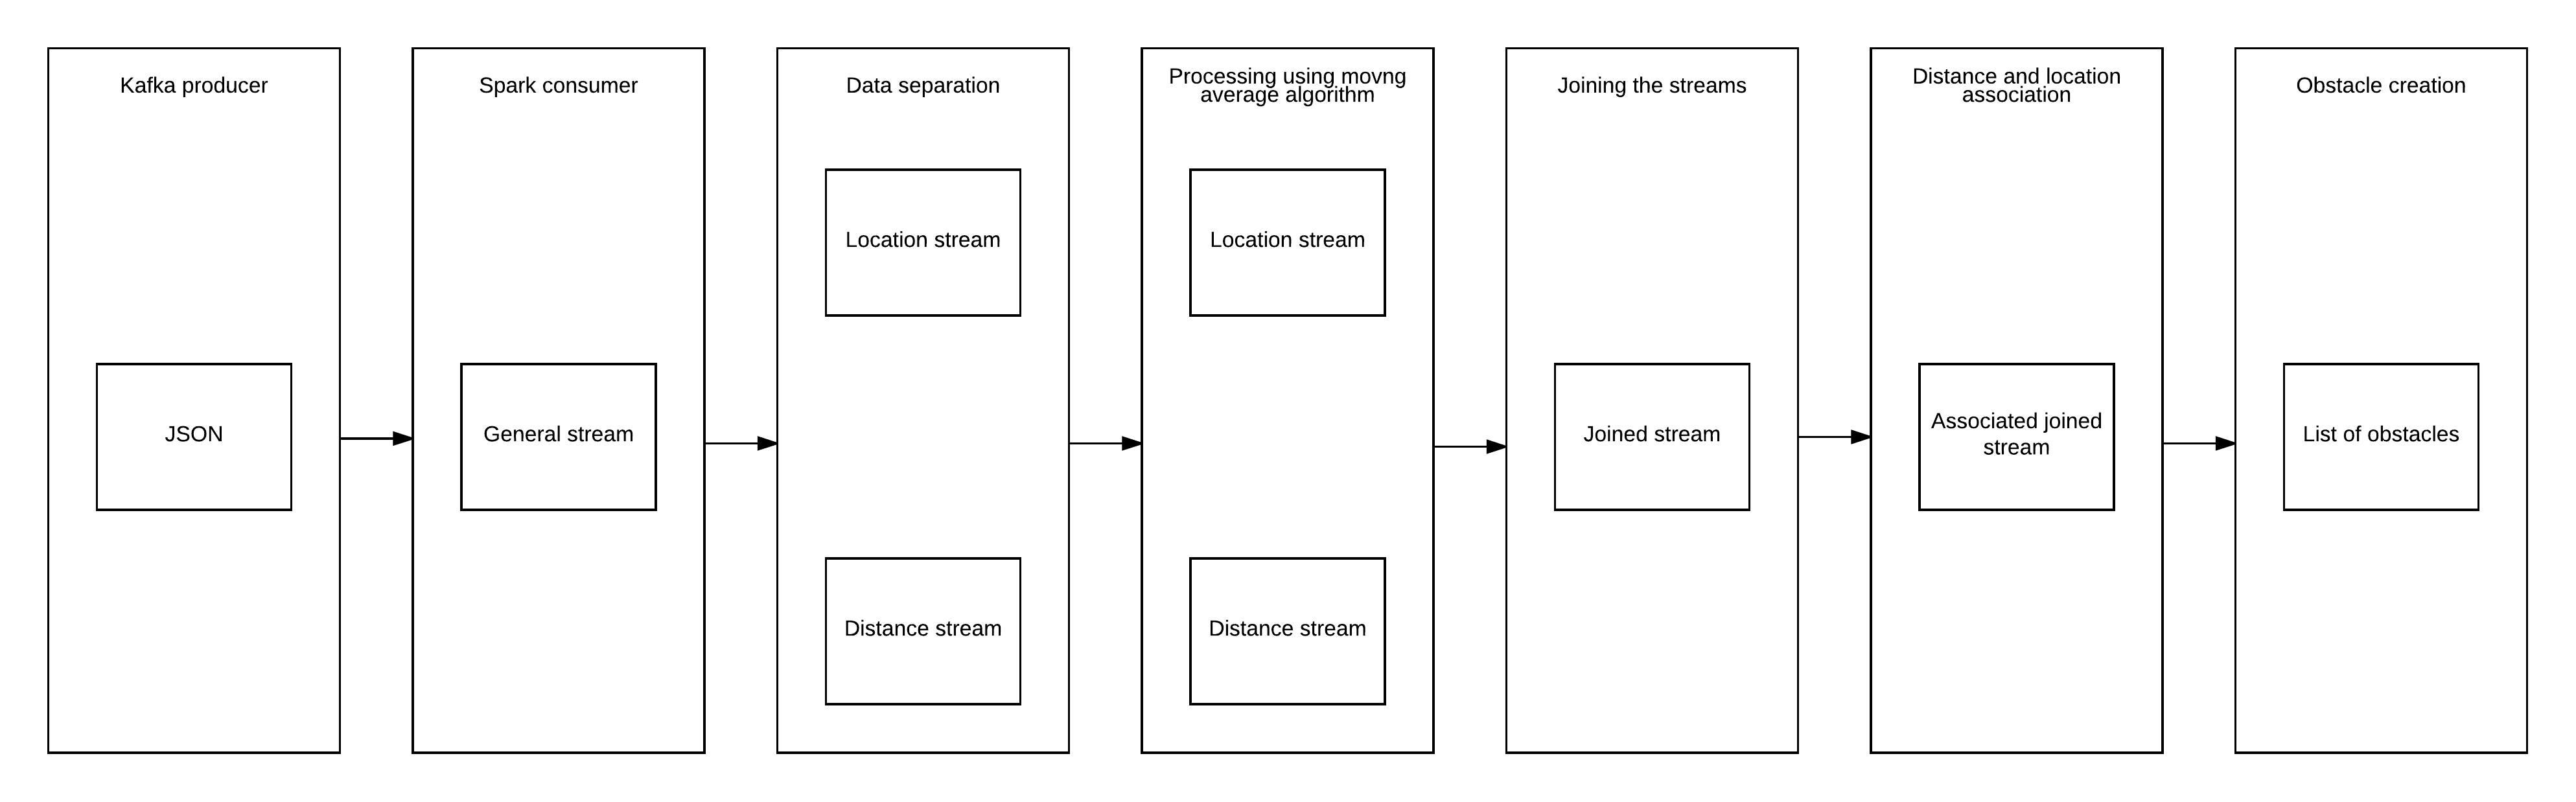
\includegraphics[width=\textwidth]{Spark}
\caption{Spark pipeline}
\label{fig:Spark pipeline}
\end{figure}

\subsection{Obstacle Query API}
To query the database an API was set up that was written in Java using the Jersey framework. The API is hosted on the same machine as Cassandra using the Tomcat web server. Upon processing by spark, a single obstacle location is stored in Cassandra with a confidence of 0 - 100. Confidence states how certain we are the obstacle would not move position with time. For example a pillar would have a higher confidence in comparison to a chair or trash can because it will hardly change its position.

\subsection{Cassandra}
The data modelling for Cassandra was fairly simple, the number of data points needed to persist an obstacle were few and clear. After setting up the Cassandra server the data model was set up through CQL and drivers with Java set up for testing and querying.

\section{Project Management}
As discussed earlier the 4 CS students are each responsible for data collection or feedback application that would be the topic of their dissertation project.
The role of the SSE team with regards to the CS students was to coordinate their efforts towards creating value for the client and to provide them with guidance with the implementation and architecture of their projects.

\subsection{Processes}
The SSE team managed their work by relying on the Scrum methodology. Work was organised into 2 week sprints and standup meetings were scheduled for communication and status updates. Mondays were set up as meeting days to synchronise with stakeholders, academic supervisors and our client. Standup meetings were held the following Tuesday which was used to re-organise and adapt the work schedule over the week to the most recent project vision of our client. Fridays were used to write reports and inform our stakeholders of the progress made. The team would hand in a weekly report and send demonstration material to the client to show progress and receive feedback.

\subsection{Testing strategy}
The testing strategy was a large consideration for the SSE team, since the many components of the architecture had different interfaces so each needed a strategy tailor made for it. In order to manage and enforce the testing strategy the team set up a continuous integration server, Jenkins, to run tests as code was pushed to Git and run unit, load and integration tests.

\subsubsection{Kafka}
The main quality requirement for the UDP socket server for the Kafka producer was the throughput. Therefore load tests were the main focus in the testing strategy for this component. Since the component uses UDP the metrics gathered were to measure number of packets processed, number of packets dropped and the processing speed of each packet from the socket and into the message queue. The team considered using unit testing and integration tests to evaluate this component but the work involved in mocking out dependencies was not the most efficient use of time. The Kafka producer should contain as little logic as possible and therefore unit tests would be of little value. Integration tests on this component would be run when testing the integration with the Spark processing component.

\subsubsection{Spark}
This component has a similar testing strategy to the Kafka component. The processing throughput is a large concern since the entire processing pipeline needs to be checked for bottlenecks so load test will need to be performed. Integration tests are also required to test if the processing is producing the correct output. Here the dependency of the processing component on the Spark environment creates real problems to unit testing. Mocking this out is a major effort so the integration tests were found to be sufficient to assure the team that the processing is producing the correct results.

\subsubsection{Obstacle API}
The obstacle REST API has several logic components that need unit testing in addition to other testing methods. The logic will be tested through unit tests and the HTTP compliance and error checks will be performed through integration tests. In addition to this some load tests will be performed to make sure the API stands up to a minimum level of load expected in our quality requirements.

\subsubsection{Indoor Atlas}
%TODO: Shuang add a discussion
The user's location collecting component based on Indoor Atlas in our project requires low latency and high accuracy. The latency will be tested by recording the time when sending the data and the time when getting the response. Overall 20 testing will be taken, and the average result is the latency. To test the accuracy, IndoorAtlas provides the average accuracy tested by their platform. Also, the actual accuracy will be measured by calculating the distance between the actual user location and the IndoorAtlas result.

\section{Evaluation}
Given the nature of the project the main success criteria is if the system can accurately determine the location of an obstacle in space based on the sensor data given. The evaluation of this fact was done by doing experiments with the actual sensor hardware, extracting the noise level, accuracy and other quality metrics and then generating sensor output based on those metrics. This generation of test data allowed us to evaluate the accuracy of our system in a controlled environment. We evaluated the robustness of our processing methods by increasing the noise in the generated sensor signal in addition to controlling the rate of data sent to the system. The throughput of the system was also evaluated by sending large amounts of sensor readings at a time and measuring response time, packet loss and transmission delay.

\subsection{Tools and Data generation}
The data was generated through a simulation script written in Python. The simulation was set up by specifying an agent, some obstacles and a set of sensors. The agent and obstacles would have a location in space and the agent had a maximum velocity, rotation speed and other movement parameters. The simulation would then be configured by laying out a path for the agent to move through while the sensors were polled to check if they would detect an obstacle. The simulation allowed for noise to be added to the sensor readings that would give a more realistic way of processing sensor data that will inherently contain error and noise.

\subsection{Performance and Scalability}
After implementing the processing pipeline the first performance test performed was to evaluate the throughput and packet loss. This was done by sending progressively larger numbers of simulated sensor readings to the pipeline and measure how it handled the load.

\begin{center}
\begin{tabularx}{\textwidth}{| X | X | X | X |} 
\hline
\# Readings & Transmission time & \# Readings/Second & Packet Loss \% \\
\hline
7400 & 2.220366535 & 3332.783071 & 1.135135135 \\
\hline
74000 & 15.81466027 & 4678.380612 & 0.7731087894 \\
\hline
740000 & 119.9508543 & 5738.18339 & 5.847595525 \\
\hline
\end{tabularx}
\label{tab:performance}
\end{center}

The results shown in table~\ref{tab:performance} show that the pipeline handled loads far beyond what was stipulated in the quality requirements, the packet loss is within acceptable limits (2\%) for over 100000 readings and the throughput was an order of magnitude higher than the goal. The quality requirements needed the pipeline to handle 100 readings per second but the load testing showed that the pipeline could handle over 5000 messages before it started to experience deteriorating performance.

\begin{figure}
\centering
\subfigure[Figure 1] {
  \label{fig:sub1}
  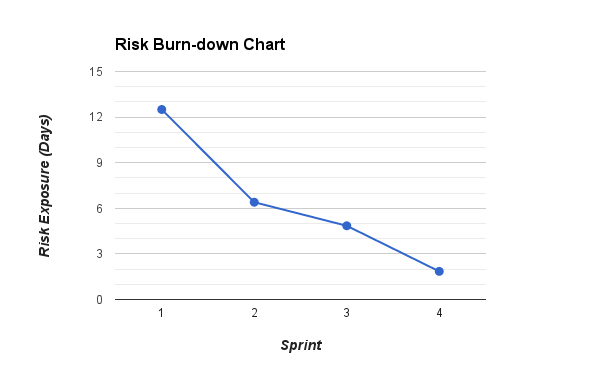
\includegraphics[width=.3\linewidth]{burndown-chart}
}
\subfigure[Figure 2] {
  \label{fig:sub1}
  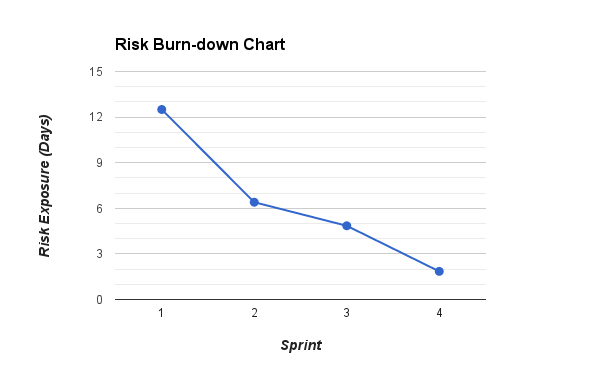
\includegraphics[width=.3\linewidth]{burndown-chart}
}
\subfigure[Figure 3] {
  \label{fig:sub1}
  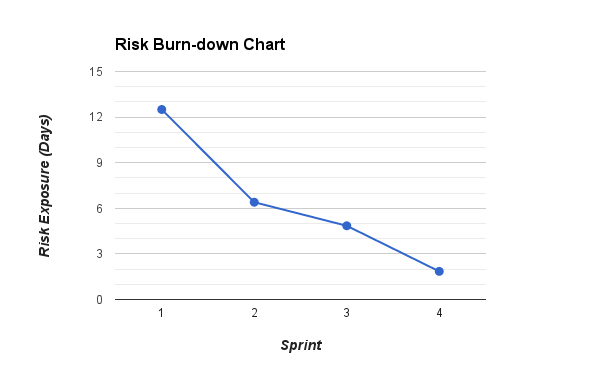
\includegraphics[width=.3\linewidth]{burndown-chart}
}
\caption{A figure with two subfigures}
\label{fig:test}

\subfigure[Figure 4] {
  \label{fig:sub1}
  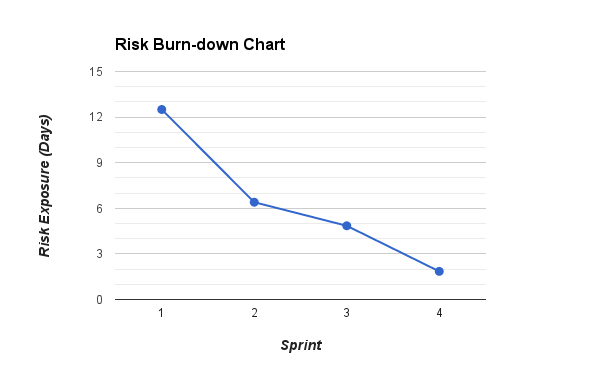
\includegraphics[width=.3\linewidth]{burndown-chart}
}
\subfigure[Figure 5] {
  \label{fig:sub1}
  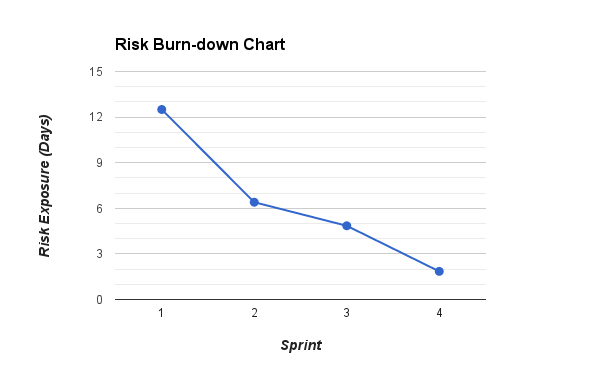
\includegraphics[width=.3\linewidth]{burndown-chart}
}
\subfigure[Figure 6] {
  \label{fig:sub1}
  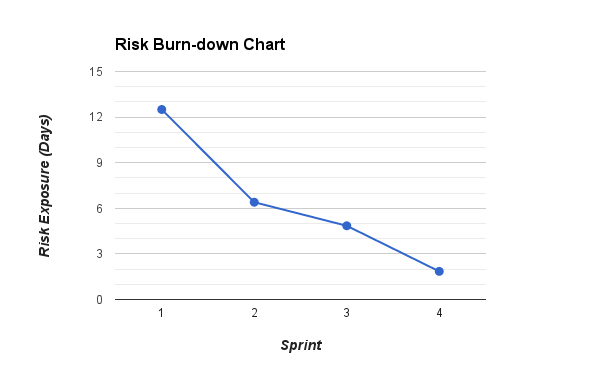
\includegraphics[width=.3\linewidth]{burndown-chart}
}
\caption{A figure with two subfigures}
\label{fig:test}
\end{figure}

\subsection{Detection accuracy}
Describe the testing scenario, the simulator and show diagrams that compare both.


\subsection{Acceptance}
%TODO: Talk about the cs students evaluation?

\section{Life cycle and Future Work}
\subsection{Current state}
The Lighthouse project now can process data from all kinds of sensors and achieves the aim of detecting obstacles. The project reaches the goal that is using low-cost and off-the-shelf sensors. Currently, the magnetic sensor in the smartphone, camera, Inferred and Ultrasound sensors works together to collect data from the indoor environment and send all the information collected to data processing component by implementing the API created by SSE team. After the processing, feedback will be shown to users in map and 3D sound. The two most important factor of performance are latency and accuracy. In our testing mentioned above, the quality of the project can fulfil the requirement of indoor real-time obstacle detection.(need to add some testing result)

\subsection{Maintenance and Scaling}
% TODO: Enumerate limitation of the product
% TODO: Describe how we can go from prototype to a running system
In the future, when the project needs to be expanded with other types of sensors, this platform can still provide the interface for communication between device and processing component. 
Although this product can fulfil the client’s requirements, it has huge performance disparity with a real industry product. Since budget and experience are limited, the capability of the project is not sufficed to support thousands of simultaneous user query.
This project can be migrated to Azure which is a Microsoft product and can provide global coverage and high availability and stability. The components of the project need to be rewritten in C\# and Azure analog technologies. First, Kafka part in this project should be replaced by Azure Event Hub. Next, Apache Storm consumes messages from the queue, which should be easy to do since Storm is hosted on HDInsight. Apache Storm is an alternative to Spark Streaming that has many of the same features but is built specifically for stream processing. Storm then performs the same processing as in the prototype stage and passes the result to a wide column store database. For the database, HBase is an alternative of Cassandra. When moving the project to Azure,  there will be an Asp.NET MVC REST API that queries HBase through the .NET SDK to expose the obstacles to the internet.

\section{Conclusions}

% TODO: identify the topic takeaway messages.
% takeaway messages describe how we one could do things differently.
% not in context of the project but rather in the context of the domain. 

% Appendix
\appendix
\section*{APPENDIX} \label{Appendix}
\setcounter{section}{1}

\appendixhead{ZHOU}

% Acknowledgments
\begin{acks}
\end{acks}  

% Bibliography
\bibliographystyle{ACM-Reference-Format-Journals}
\bibliography{GroupReport-bibfile}

% History dates
%\received{February 2007}{March 2009}{June 2009}

% Electronic Appendix
\elecappendix

\medskip

\section{This is an example of Appendix section head}


\section{Appendix section head}

\subsection{Architecture cost analysis}
\label{ArchitectureCost}

\end{document}



